Quelle: \href{http://drops.dagstuhl.de/opus/volltexte/2015/4944/pdf/44.pdf}{Visibly Counter Languages
and Constant Depth Circuits}

Was wir von reg. Sprachen wissen:
\begin{itemize}
\item $REG$ ist $NC^1$-vollst.
\item $REG\cap AC^0 = FO[Reg.]$
	= quasi aper. $\gamma:\Sigma^*\to Synt(L)$
\item $REG L \notin AC^0 \Rightarrow L \text{ ist } ACC^0 \text{-schwer}$
\end{itemize}
$AC^0 \subsetneq ACC_k^0 \subseteq TC^0 \subseteq NC^1 \subseteq L \subseteq NL$\\
\vspace{1cm}\\
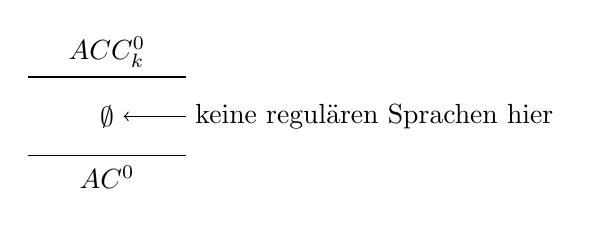
\begin{tikzpicture}
\draw (0,1) -- (2,1) node[midway, above] (acc) {$ACC_k^0$};
\node at (1,0.5) (empty) {$\emptyset$};
\draw [<-] (empty) -- (2,0.5) node [anchor= west] {keine regulären Sprachen hier};
\draw (0,0) -- (2,0) node[midway, below] (ac0) {$AC^0$};
\end{tikzpicture}\\
Dichotomie\\
VPL auch $NC^1$-vollständig, also auch $VCL$.

\section{Definition}
$k-VCA\quad\mathcal{A} = (Q, q_0, E, \Sigma, \delta_0, \dots, \delta_k)$\\
$$\delta_i = Q \times \Sigma \to \Sigma$$
Akz: Endzust. in Lauf erreichbar: $\delta_{min}(m, \Delta(w))$ wird angewandt, nachdem $w$ gelesen wurde.\\
\begin{tikzpicture}
\draw[->] (0,0) -- (0,3);
\node at (0,1) [anchor=east] (m) {$\delta_m$};
\draw[dotted] (m) -- (4,1);
\draw[gray!50] (0,1) -- (1,2) -- (2,1) -- (3,3) -- (4,1);
\fill[gray!20, pattern=north east lines] (0,1) -- (1,2) -- (2,1) -- (3,3) -- (4,1) -- cycle;
\draw[->] (0,0) -- (4,0);
\end{tikzpicture}\\
$$\Delta(w) = |w|_{call} - |w|_{return}$$
Bsp.: $a^nb^n \to 1-VCL$\\
$a^nb^{n-3}a^mb^{m+3} \to 4-VCA$

